% Options for packages loaded elsewhere
% Options for packages loaded elsewhere
\PassOptionsToPackage{unicode}{hyperref}
\PassOptionsToPackage{hyphens}{url}
\PassOptionsToPackage{dvipsnames,svgnames,x11names}{xcolor}
%
\documentclass[
  letterpaper,
  DIV=11,
  numbers=noendperiod]{scrartcl}
\usepackage{xcolor}
\usepackage{amsmath,amssymb}
\setcounter{secnumdepth}{-\maxdimen} % remove section numbering
\usepackage{iftex}
\ifPDFTeX
  \usepackage[T1]{fontenc}
  \usepackage[utf8]{inputenc}
  \usepackage{textcomp} % provide euro and other symbols
\else % if luatex or xetex
  \usepackage{unicode-math} % this also loads fontspec
  \defaultfontfeatures{Scale=MatchLowercase}
  \defaultfontfeatures[\rmfamily]{Ligatures=TeX,Scale=1}
\fi
\usepackage{lmodern}
\ifPDFTeX\else
  % xetex/luatex font selection
\fi
% Use upquote if available, for straight quotes in verbatim environments
\IfFileExists{upquote.sty}{\usepackage{upquote}}{}
\IfFileExists{microtype.sty}{% use microtype if available
  \usepackage[]{microtype}
  \UseMicrotypeSet[protrusion]{basicmath} % disable protrusion for tt fonts
}{}
\makeatletter
\@ifundefined{KOMAClassName}{% if non-KOMA class
  \IfFileExists{parskip.sty}{%
    \usepackage{parskip}
  }{% else
    \setlength{\parindent}{0pt}
    \setlength{\parskip}{6pt plus 2pt minus 1pt}}
}{% if KOMA class
  \KOMAoptions{parskip=half}}
\makeatother
% Make \paragraph and \subparagraph free-standing
\makeatletter
\ifx\paragraph\undefined\else
  \let\oldparagraph\paragraph
  \renewcommand{\paragraph}{
    \@ifstar
      \xxxParagraphStar
      \xxxParagraphNoStar
  }
  \newcommand{\xxxParagraphStar}[1]{\oldparagraph*{#1}\mbox{}}
  \newcommand{\xxxParagraphNoStar}[1]{\oldparagraph{#1}\mbox{}}
\fi
\ifx\subparagraph\undefined\else
  \let\oldsubparagraph\subparagraph
  \renewcommand{\subparagraph}{
    \@ifstar
      \xxxSubParagraphStar
      \xxxSubParagraphNoStar
  }
  \newcommand{\xxxSubParagraphStar}[1]{\oldsubparagraph*{#1}\mbox{}}
  \newcommand{\xxxSubParagraphNoStar}[1]{\oldsubparagraph{#1}\mbox{}}
\fi
\makeatother


\usepackage{longtable,booktabs,array}
\usepackage{calc} % for calculating minipage widths
% Correct order of tables after \paragraph or \subparagraph
\usepackage{etoolbox}
\makeatletter
\patchcmd\longtable{\par}{\if@noskipsec\mbox{}\fi\par}{}{}
\makeatother
% Allow footnotes in longtable head/foot
\IfFileExists{footnotehyper.sty}{\usepackage{footnotehyper}}{\usepackage{footnote}}
\makesavenoteenv{longtable}
\usepackage{graphicx}
\makeatletter
\newsavebox\pandoc@box
\newcommand*\pandocbounded[1]{% scales image to fit in text height/width
  \sbox\pandoc@box{#1}%
  \Gscale@div\@tempa{\textheight}{\dimexpr\ht\pandoc@box+\dp\pandoc@box\relax}%
  \Gscale@div\@tempb{\linewidth}{\wd\pandoc@box}%
  \ifdim\@tempb\p@<\@tempa\p@\let\@tempa\@tempb\fi% select the smaller of both
  \ifdim\@tempa\p@<\p@\scalebox{\@tempa}{\usebox\pandoc@box}%
  \else\usebox{\pandoc@box}%
  \fi%
}
% Set default figure placement to htbp
\def\fps@figure{htbp}
\makeatother





\setlength{\emergencystretch}{3em} % prevent overfull lines

\providecommand{\tightlist}{%
  \setlength{\itemsep}{0pt}\setlength{\parskip}{0pt}}



 


\KOMAoption{captions}{tableheading}
\makeatletter
\@ifpackageloaded{tcolorbox}{}{\usepackage[skins,breakable]{tcolorbox}}
\@ifpackageloaded{fontawesome5}{}{\usepackage{fontawesome5}}
\definecolor{quarto-callout-color}{HTML}{909090}
\definecolor{quarto-callout-note-color}{HTML}{0758E5}
\definecolor{quarto-callout-important-color}{HTML}{CC1914}
\definecolor{quarto-callout-warning-color}{HTML}{EB9113}
\definecolor{quarto-callout-tip-color}{HTML}{00A047}
\definecolor{quarto-callout-caution-color}{HTML}{FC5300}
\definecolor{quarto-callout-color-frame}{HTML}{acacac}
\definecolor{quarto-callout-note-color-frame}{HTML}{4582ec}
\definecolor{quarto-callout-important-color-frame}{HTML}{d9534f}
\definecolor{quarto-callout-warning-color-frame}{HTML}{f0ad4e}
\definecolor{quarto-callout-tip-color-frame}{HTML}{02b875}
\definecolor{quarto-callout-caution-color-frame}{HTML}{fd7e14}
\makeatother
\makeatletter
\@ifpackageloaded{caption}{}{\usepackage{caption}}
\AtBeginDocument{%
\ifdefined\contentsname
  \renewcommand*\contentsname{Contents}
\else
  \newcommand\contentsname{Contents}
\fi
\ifdefined\listfigurename
  \renewcommand*\listfigurename{List of Figures}
\else
  \newcommand\listfigurename{List of Figures}
\fi
\ifdefined\listtablename
  \renewcommand*\listtablename{List of Tables}
\else
  \newcommand\listtablename{List of Tables}
\fi
\ifdefined\figurename
  \renewcommand*\figurename{Figure}
\else
  \newcommand\figurename{Figure}
\fi
\ifdefined\tablename
  \renewcommand*\tablename{Table}
\else
  \newcommand\tablename{Table}
\fi
}
\@ifpackageloaded{float}{}{\usepackage{float}}
\floatstyle{ruled}
\@ifundefined{c@chapter}{\newfloat{codelisting}{h}{lop}}{\newfloat{codelisting}{h}{lop}[chapter]}
\floatname{codelisting}{Listing}
\newcommand*\listoflistings{\listof{codelisting}{List of Listings}}
\makeatother
\makeatletter
\makeatother
\makeatletter
\@ifpackageloaded{caption}{}{\usepackage{caption}}
\@ifpackageloaded{subcaption}{}{\usepackage{subcaption}}
\makeatother
\usepackage{bookmark}
\IfFileExists{xurl.sty}{\usepackage{xurl}}{} % add URL line breaks if available
\urlstyle{same}
\hypersetup{
  pdftitle={Copernicus Sentinel Data \& Philippine EO Ecosystem},
  pdfauthor={Stylianos Kotsopoulos},
  colorlinks=true,
  linkcolor={blue},
  filecolor={Maroon},
  citecolor={Blue},
  urlcolor={Blue},
  pdfcreator={LaTeX via pandoc}}


\title{Copernicus Sentinel Data \& Philippine EO Ecosystem}
\usepackage{etoolbox}
\makeatletter
\providecommand{\subtitle}[1]{% add subtitle to \maketitle
  \apptocmd{\@title}{\par {\large #1 \par}}{}{}
}
\makeatother
\subtitle{CoPhil EO AI/ML Training - Day 1, Session 1}
\author{Stylianos Kotsopoulos}
\date{}
\begin{document}
\maketitle


\section{Welcome}\label{welcome}

\subsection{Course Introduction}\label{course-introduction}

\textbf{4-Day Advanced Training}

\begin{itemize}
\tightlist
\item
  AI/ML for Earth Observation
\item
  Philippine EO Professionals
\item
  Focus: DRR, CCA, NRM
\item
  Online format
\end{itemize}

\textbf{Today's Goals}

\begin{itemize}
\tightlist
\item
  Understand Copernicus data
\item
  Explore Philippine EO ecosystem
\item
  Learn AI/ML fundamentals
\item
  Hands-on Python and GEE
\end{itemize}

Welcome participants to the 4-day advanced training. Emphasize that this
is part of the EU-Philippines partnership and will provide practical
skills for disaster risk reduction, climate change adaptation, and
natural resource management.

\subsection{EU Global Gateway
Initiative}\label{eu-global-gateway-initiative}

\begin{itemize}
\tightlist
\item
  EU-Philippines space cooperation flagship
\item
  Building strong partnerships
\item
  Smart, clean, secure digital links
\item
  Strengthening health, education, research systems globally
\end{itemize}

\begin{center}

\includegraphics[width=0.6\linewidth,height=\textheight,keepaspectratio]{images/eu_global_gateway.png}
\end{center}

The Global Gateway strategy represents the EU's commitment to building
partnerships that boost smart, clean and secure infrastructure globally.
CoPhil is a unique flagship initiative within this framework.

\subsection{CoPhil Programme Overview}\label{cophil-programme-overview}

\textbf{Mission}

Support Philippine Space Agency (PhilSA) and DOST to improve use of
Earth Observation data for:

\begin{itemize}
\tightlist
\item
  Disaster Risk Reduction (DRR)
\item
  Climate Change Adaptation (CCA)
\item
  Natural Resource Management (NRM)
\end{itemize}

\textbf{Key Outputs}

\begin{itemize}
\tightlist
\item
  Copernicus Mirror Site
\item
  Digital Space Campus
\item
  Capacity building
\item
  Pilot services
\end{itemize}

CoPhil is an EU-funded Technical Assistance programme positioning the
Philippines as a pioneer in the EU's international cooperation on
Copernicus.

\subsection{PhilSA \& DOST Partnership}\label{philsa-dost-partnership}

\textbf{Philippine Space Agency}

\includegraphics[width=2.08333in,height=\textheight,keepaspectratio]{images/philsa_logo.png}

\begin{itemize}
\tightlist
\item
  Established 2019
\item
  Central civilian space agency
\item
  Space+ Data Dashboard
\item
  Co-chair of CoPhil
\end{itemize}

\textbf{Department of Science and Technology}

\includegraphics[width=2.08333in,height=\textheight,keepaspectratio]{images/dost_logo.png}

\begin{itemize}
\tightlist
\item
  ASTI AI initiatives
\item
  SkAI-Pinas program
\item
  National AI investments
\item
  Co-chair of CoPhil
\end{itemize}

Both PhilSA and DOST are co-chairs of the CoPhil programme,
demonstrating strong national commitment to building EO and AI capacity.

\subsection{Session 1 Roadmap}\label{session-1-roadmap}

\begin{enumerate}
\def\labelenumi{\arabic{enumi}.}
\tightlist
\item
  Copernicus Programme Overview
\item
  Sentinel-1 Mission (SAR)
\item
  Sentinel-2 Mission (Optical)
\item
  Data Access Methods
\item
  Philippine EO Ecosystem
\item
  CoPhil Infrastructure
\end{enumerate}

\textbf{Duration:} 2 hours

This session provides the foundation for understanding where EO data
comes from and how Philippine agencies complement Copernicus data.

\section{Part 1: The Copernicus
Programme}\label{part-1-the-copernicus-programme}

\subsection{What is Copernicus?}\label{what-is-copernicus}

\textbf{Europe's Eyes on Earth}

\begin{itemize}
\tightlist
\item
  EU flagship Earth Observation program
\item
  Family of Sentinel satellites
\item
  \textbf{Free and open data policy}
\item
  Operational since 2014
\end{itemize}

\includegraphics[width=1\linewidth,height=\textheight,keepaspectratio]{images/copernicus_overview.jpg}

\textbf{``Looking at our planet and its environment for the benefit of
all European citizens''}

Copernicus is the European Union's Earth Observation program, providing
free and open satellite data globally. It comprises a fleet of Sentinel
satellites designed for environmental monitoring.

\begin{center}\rule{0.5\linewidth}{0.5pt}\end{center}

\subsection{Copernicus Programme
Architecture}\label{copernicus-programme-architecture}

\begin{figure}[H]

{\centering 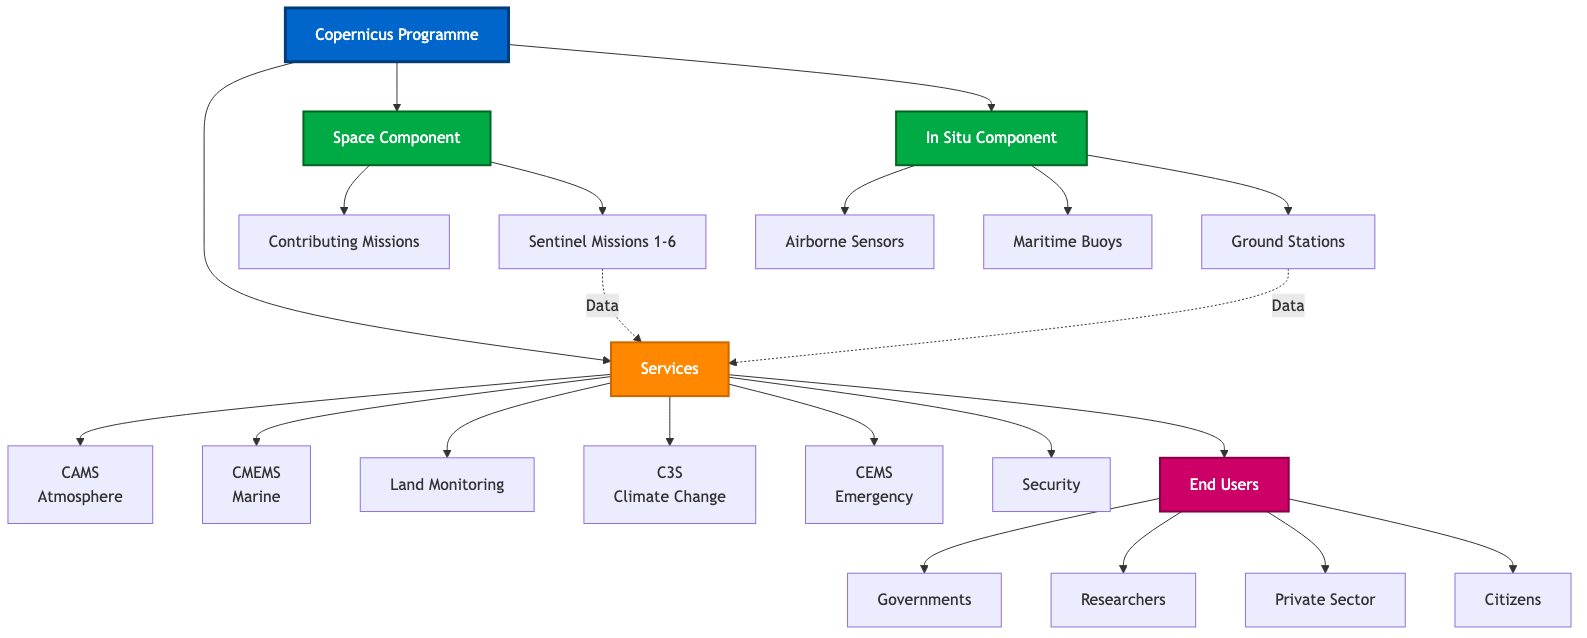
\includegraphics[width=0.9\linewidth,height=\textheight,keepaspectratio]{../../diagrams_export/diagram_001_day1_sessions_session1_1.png}

}

\caption{Copernicus Programme Structure showing Space Component,
Services, and End Users}

\end{figure}%

This diagram shows the complete Copernicus architecture: the space
component with Sentinel missions, in-situ data sources, the six core
services (CAMS, CMEMS, Land, Climate, Emergency, Security), and the
various end-user categories.

\begin{center}\rule{0.5\linewidth}{0.5pt}\end{center}

\subsection{The Sentinel Family}\label{the-sentinel-family}

\textbf{Sentinel-1} (SAR)

\begin{itemize}
\tightlist
\item
  C-band radar imaging
\item
  All-weather, day/night
\item
  1A operational, \textbf{1C launched Dec 2024}
\item
  6-day repeat (dual constellation)
\end{itemize}

\textbf{Sentinel-2} (Optical)

\begin{itemize}
\tightlist
\item
  Multispectral imaging
\item
  13 spectral bands
\item
  2A, 2B, \textbf{2C operational Jan 2025}
\item
  5-day repeat (three satellites)
\end{itemize}

\textbf{Sentinel-3} (Ocean/Land)

\begin{itemize}
\tightlist
\item
  Ocean and land monitoring
\item
  Sea surface temperature
\item
  Ocean color, vegetation
\end{itemize}

\textbf{Sentinel-5P} (Atmosphere)

\begin{itemize}
\tightlist
\item
  Air quality monitoring
\item
  Atmospheric composition
\end{itemize}

\textbf{Timing:} 4 minutes

\textbf{Key Points:} - Six Sentinel missions operational (1, 2, 3, 5P,
6) with 4, 7-12 planned - \textbf{2025 Update:} Sentinel-1C launched
December 2024, restoring 6-day global repeat - \textbf{2025 Update:}
Sentinel-2C operational January 2025, creating 3-satellite constellation
with 5-day repeat - Today we focus on Sentinel-1 and Sentinel-2 - most
relevant for Philippine DRR/CCA/NRM - Sentinel-3 important for
marine/coastal applications - Sentinel-5P monitors air pollution (useful
for Manila air quality)

\textbf{Transition:} ``These missions generate petabytes of free data.
Let's see how this data is used\ldots{}''

\subsection{Copernicus Applications}\label{copernicus-applications}

\begin{center}
\includegraphics[width=0.8\linewidth,height=\textheight,keepaspectratio]{images/copernicus_applications.png}
\end{center}

\textbf{Emergency Management}

\begin{itemize}
\tightlist
\item
  Flood mapping
\item
  Fire detection
\item
  Disaster response
\end{itemize}

\textbf{Climate \& Environment}

\begin{itemize}
\tightlist
\item
  Deforestation monitoring
\item
  Agricultural monitoring
\item
  Water quality assessment
\end{itemize}

Copernicus supports applications in emergency management, health care,
agriculture, and environment, with crucial impact on society, climate,
and economy.

\section{Sentinel-1: SAR Mission}\label{sentinel-1-sar-mission}

\subsection{Sentinel-1 Overview}\label{sentinel-1-overview}

\textbf{Mission Configuration (2025)}

\begin{itemize}
\tightlist
\item
  \textbf{Sensor:} C-band Synthetic Aperture Radar
\item
  \textbf{Satellites:} 1A, \textbf{1C (operational 2025)}
\item
  \textbf{Orbit:} Polar sun-synchronous
\item
  \textbf{All-weather, day/night capability}
\end{itemize}

\includegraphics[width=1\linewidth,height=\textheight,keepaspectratio]{images/sentinel1_satellite.jpg}

\textbf{Key Advantage:} Penetrates clouds and works at night

Sentinel-1 is a radar imaging mission with C-band SAR enabling
all-weather, day-and-night observations unaffected by clouds - crucial
in tropical regions like the Philippines.

\subsection{Sentinel-1 Technical
Specifications}\label{sentinel-1-technical-specifications}

\begin{longtable}[]{@{}ll@{}}
\toprule\noalign{}
\textbf{Parameter} & \textbf{Value} \\
\midrule\noalign{}
\endhead
\bottomrule\noalign{}
\endlastfoot
\textbf{Sensor Type} & C-band SAR (5.405 GHz) \\
\textbf{Revisit Time} & 6-12 days (constellation) \\
\textbf{Swath Width} & 250 km (IW mode) \\
\textbf{Spatial Resolution} & 5m × 20m (IW mode) \\
\textbf{Polarization} & VV + VH or HH + HV \\
\textbf{Orbit} & 693 km altitude \\
\end{longtable}

Sentinel-1 operates in Interferometric Wide (IW) mode with
\textasciitilde5m by 20m spatial resolution. With two satellites, the
revisit cycle is 6 days globally. Note: Sentinel-1B became inoperative
in 2022; Sentinel-1C launched in 2024 to restore 6-day revisit.

\subsection{SAR: How It Works}\label{sar-how-it-works}

\begin{center}
\includegraphics[width=0.7\linewidth,height=\textheight,keepaspectratio]{images/sar_principle.png}
\end{center}

\begin{enumerate}
\def\labelenumi{\arabic{enumi}.}
\tightlist
\item
  Satellite sends \textbf{microwave pulses} to Earth
\item
  Signal \textbf{reflects} from surface
\item
  Sensor measures \textbf{backscatter intensity}
\item
  Different surfaces = different backscatter
\end{enumerate}

SAR satellites send microwave signals and measure the backscatter. Water
appears dark (low backscatter), urban areas appear bright (strong
backscatter), and vegetation shows moderate backscatter.

\subsection{Sentinel-1 Polarization}\label{sentinel-1-polarization}

\textbf{What is Polarization?}

\begin{itemize}
\tightlist
\item
  Orientation of radar wave
\item
  VV: Vertical send/receive
\item
  VH: Vertical send/Horizontal receive
\item
  HH: Horizontal send/receive
\end{itemize}

\textbf{Applications}

\begin{itemize}
\tightlist
\item
  \textbf{VV:} Good for water/flood mapping
\item
  \textbf{VH:} Sensitive to volume scattering (vegetation)
\item
  \textbf{VV/VH Ratio:} Discriminates surface types
\end{itemize}

\begin{center}
\includegraphics[width=0.6\linewidth,height=\textheight,keepaspectratio]{images/polarization_comparison.jpg}
\end{center}

Sentinel-1 IW mode over land typically provides VV and VH polarizations.
Different polarizations are sensitive to different surface
characteristics.

\subsection{Backscatter Characteristics by
Target}\label{backscatter-characteristics-by-target}

\begin{longtable}[]{@{}llll@{}}
\toprule\noalign{}
\textbf{Surface Type} & \textbf{Backscatter} & \textbf{Appearance} &
\textbf{Reason} \\
\midrule\noalign{}
\endhead
\bottomrule\noalign{}
\endlastfoot
\textbf{Water (smooth)} & Very Low & Dark/Black & Specular reflection \\
\textbf{Urban/Buildings} & Very High & Bright White & Corner
reflectors \\
\textbf{Forest/Vegetation} & Medium-High & Gray & Volume scattering \\
\textbf{Agricultural Fields} & Medium & Light Gray & Surface
roughness \\
\textbf{Bare Soil (dry)} & Low-Medium & Dark Gray & Smooth surface \\
\textbf{Bare Soil (wet)} & Medium & Medium Gray & Increased
dielectric \\
\end{longtable}

\textbf{Key Insight:} Water appears dark, structures appear bright - the
basis for flood mapping!

Understanding backscatter is crucial for interpreting SAR imagery.
Smooth surfaces (water) reflect signals away = dark. Rough surfaces and
structures reflect signals back = bright.

\subsection{Sentinel-1 Imaging Modes}\label{sentinel-1-imaging-modes}

\textbf{Interferometric Wide Swath (IW)} - \textbf{250 km swath} - 5m ×
20m resolution - \textbf{Default over land} - Philippine standard mode

\textbf{Extra Wide Swath (EW)} - 400 km swath - 20m × 40m resolution -
Maritime/polar regions

\textbf{Strip Map (SM)} - 80 km swath - 5m × 5m resolution - Emergency
response - High detail needed

\textbf{Wave (WV)} - Ocean waves - Not used for land

Interferometric Wide (IW) mode is used over land and provides the best
balance of resolution and coverage. All Philippine acquisitions use IW
mode.

\subsection{Sentinel-1 Data Products}\label{sentinel-1-data-products}

\textbf{Level-1 GRD (Ground Range Detected)}

\begin{itemize}
\tightlist
\item
  Multi-looked (reduced speckle)
\item
  Projected to ground range
\item
  \textbf{Most commonly used}
\item
  Faster to process
\item
  Smaller file size
\item
  \textbf{Applications:}

  \begin{itemize}
  \tightlist
  \item
    Change detection
  \item
    Classification
  \item
    Flood mapping
  \item
    Ship detection
  \end{itemize}
\end{itemize}

\textbf{Level-1 SLC (Single Look Complex)}

\begin{itemize}
\tightlist
\item
  Preserves phase information
\item
  Complex-valued pixels
\item
  Required for InSAR
\item
  Larger files
\item
  \textbf{Applications:}

  \begin{itemize}
  \tightlist
  \item
    Ground deformation
  \item
    Interferometry
  \item
    Coherence analysis
  \item
    Subsidence monitoring
  \end{itemize}
\end{itemize}

For most applications including flood mapping and land cover, GRD
products are sufficient. SLC products are needed for advanced
interferometric applications like volcano monitoring.

\subsection{GRD vs SLC - Which to
Choose?}\label{grd-vs-slc---which-to-choose}

\begin{longtable}[]{@{}lll@{}}
\toprule\noalign{}
\textbf{Factor} & \textbf{GRD} & \textbf{SLC} \\
\midrule\noalign{}
\endhead
\bottomrule\noalign{}
\endlastfoot
\textbf{Use Case} & Most applications & Interferometry only \\
\textbf{Processing} & Ready to use & Complex processing \\
\textbf{File Size} & \textasciitilde1 GB & \textasciitilde4 GB \\
\textbf{Speckle} & Reduced & Full speckle \\
\textbf{Phase} & Not preserved & Preserved \\
\textbf{Typical User} & Most analysts & Advanced specialists \\
\end{longtable}

\textbf{For this training and most Philippine applications: Use GRD}

Unless you specifically need interferometry (earthquake/volcano
deformation), always use GRD products. They're easier to work with and
sufficient for 90\% of applications.

\begin{center}\rule{0.5\linewidth}{0.5pt}\end{center}

\subsection{Sentinel-1 Pre-Processing ``Under the
Hood''}\label{sentinel-1-pre-processing-under-the-hood}

\begin{tcolorbox}[enhanced jigsaw, left=2mm, opacityback=0, toprule=.15mm, breakable, title=\textcolor{quarto-callout-note-color}{\faInfo}\hspace{0.5em}{What Happens Before You See SAR Data?}, colbacktitle=quarto-callout-note-color!10!white, arc=.35mm, titlerule=0mm, colback=white, bottomtitle=1mm, colframe=quarto-callout-note-color-frame, leftrule=.75mm, toptitle=1mm, rightrule=.15mm, bottomrule=.15mm, opacitybacktitle=0.6, coltitle=black]

For this training, we use \textbf{pre-processed Sentinel-1 GRD data}.
Here's what happens ``under the hood'':

\end{tcolorbox}

\textbf{S1 Processing Pipeline:}

\begin{enumerate}
\def\labelenumi{\arabic{enumi}.}
\tightlist
\item
  \textbf{GRD Download} → Raw ground-range detected amplitude
\item
  \textbf{Radiometric Calibration} → Convert to backscatter coefficient
  (σ⁰)
\item
  \textbf{Terrain Correction (RTC)} → Remove topographic distortions
  using DEM
\item
  \textbf{Speckle Filtering} → Reduce SAR noise (Lee, Refined Lee, or
  Gamma-MAP filters)
\item
  \textbf{Conversion to dB} → γ⁰ (gamma-naught) in decibels for visual
  interpretation
\item
  \textbf{Tiling/Clipping} → Extract area of interest
\end{enumerate}

\textbf{For Day 3 flood mapping labs:} We provide analysis-ready patches
with these steps already applied

\textbf{P0 IMPROVEMENT APPLIED:} Explicit S1 pre-processing assumptions
before U-Net flood lab (Day 3).

\textbf{Key Teaching Points:} - Participants need to understand what
``analysis-ready'' means - RTC removes terrain effects - critical in
mountainous Philippines - Gamma-naught (γ⁰) in dB is standard for land
applications - Speckle filtering is essential but can blur edges - These
steps are computationally intensive - we pre-process for efficiency

\textbf{Timing:} 3 minutes

\textbf{Transition:} ``Now let's look at Sentinel-2 optical
data\ldots{}''

\subsection{Sentinel-1 Applications}\label{sentinel-1-applications}

\textbf{Flood Mapping}

\begin{figure}[H]

{\centering 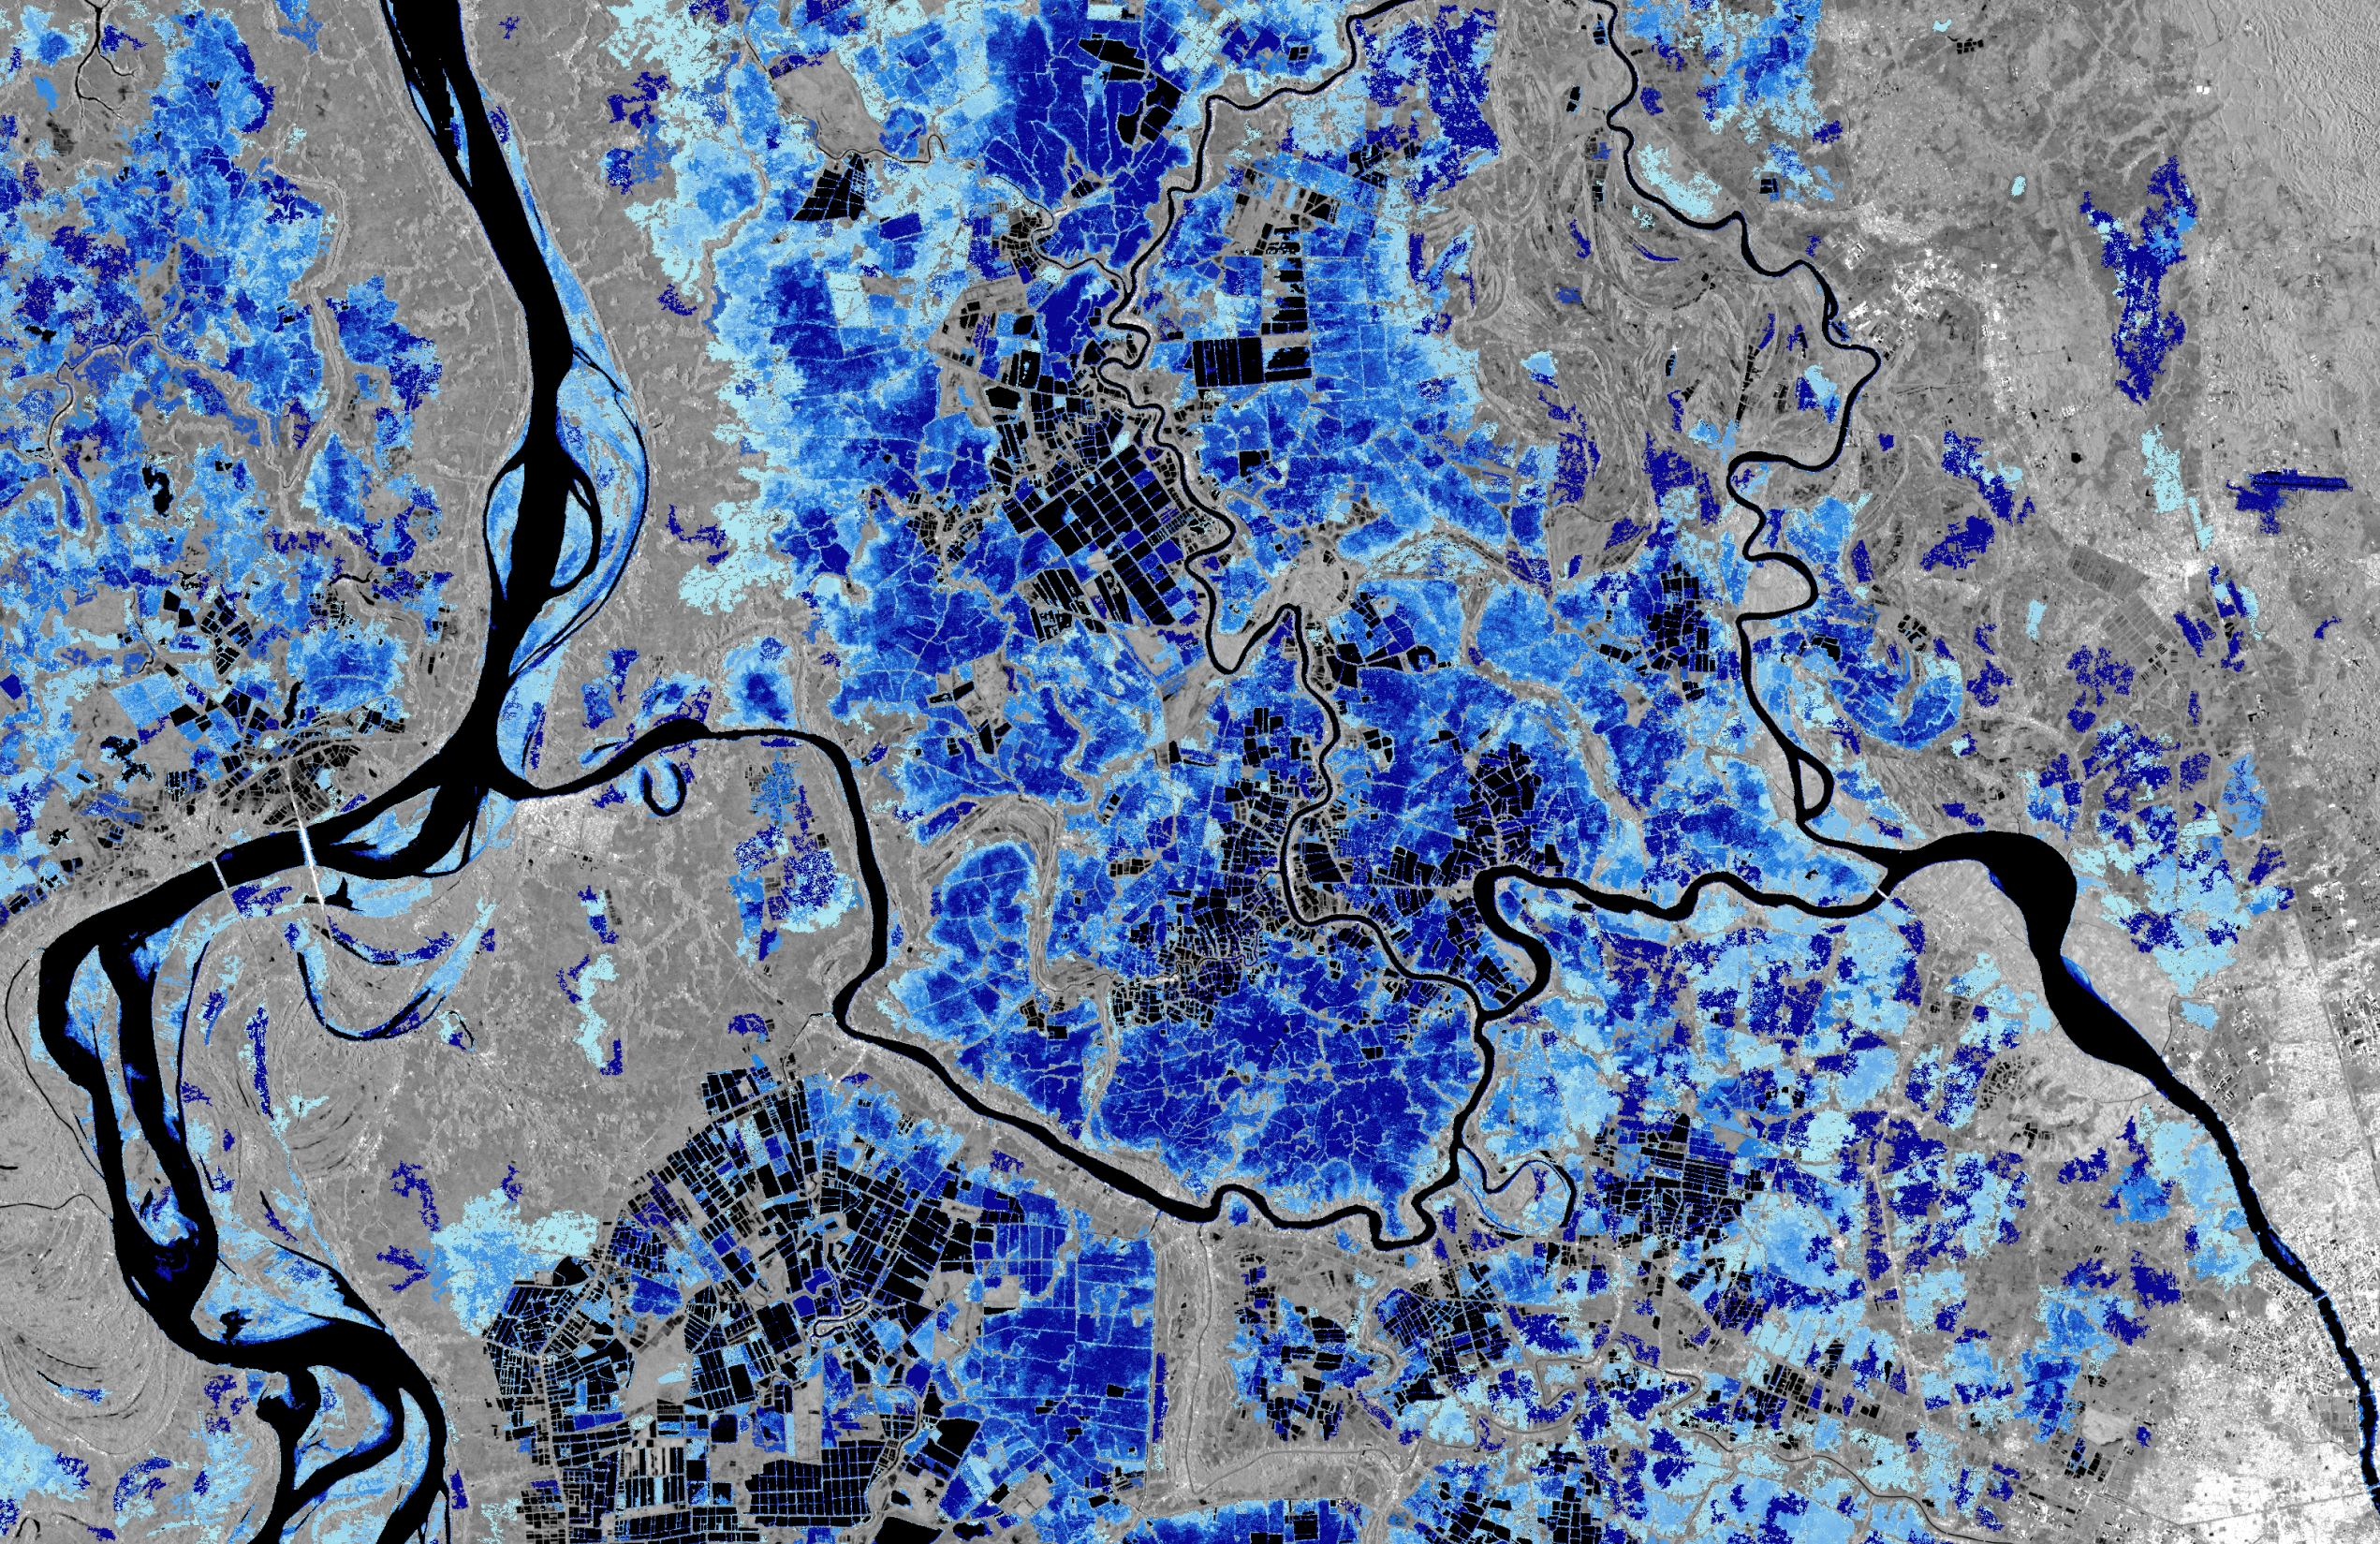
\includegraphics[width=1\linewidth,height=3.64583in]{images/Copernicus_Sentinel-1_flood_monitoring.jpg}

}

\caption{Copernicus Sentinel-1 Flood Monitoring}

\end{figure}%

\begin{itemize}
\tightlist
\item
  Water appears dark in SAR
\item
  Works through clouds
\item
  Near real-time monitoring
\end{itemize}

\textbf{Deformation Monitoring}

\begin{figure}[H]

{\centering 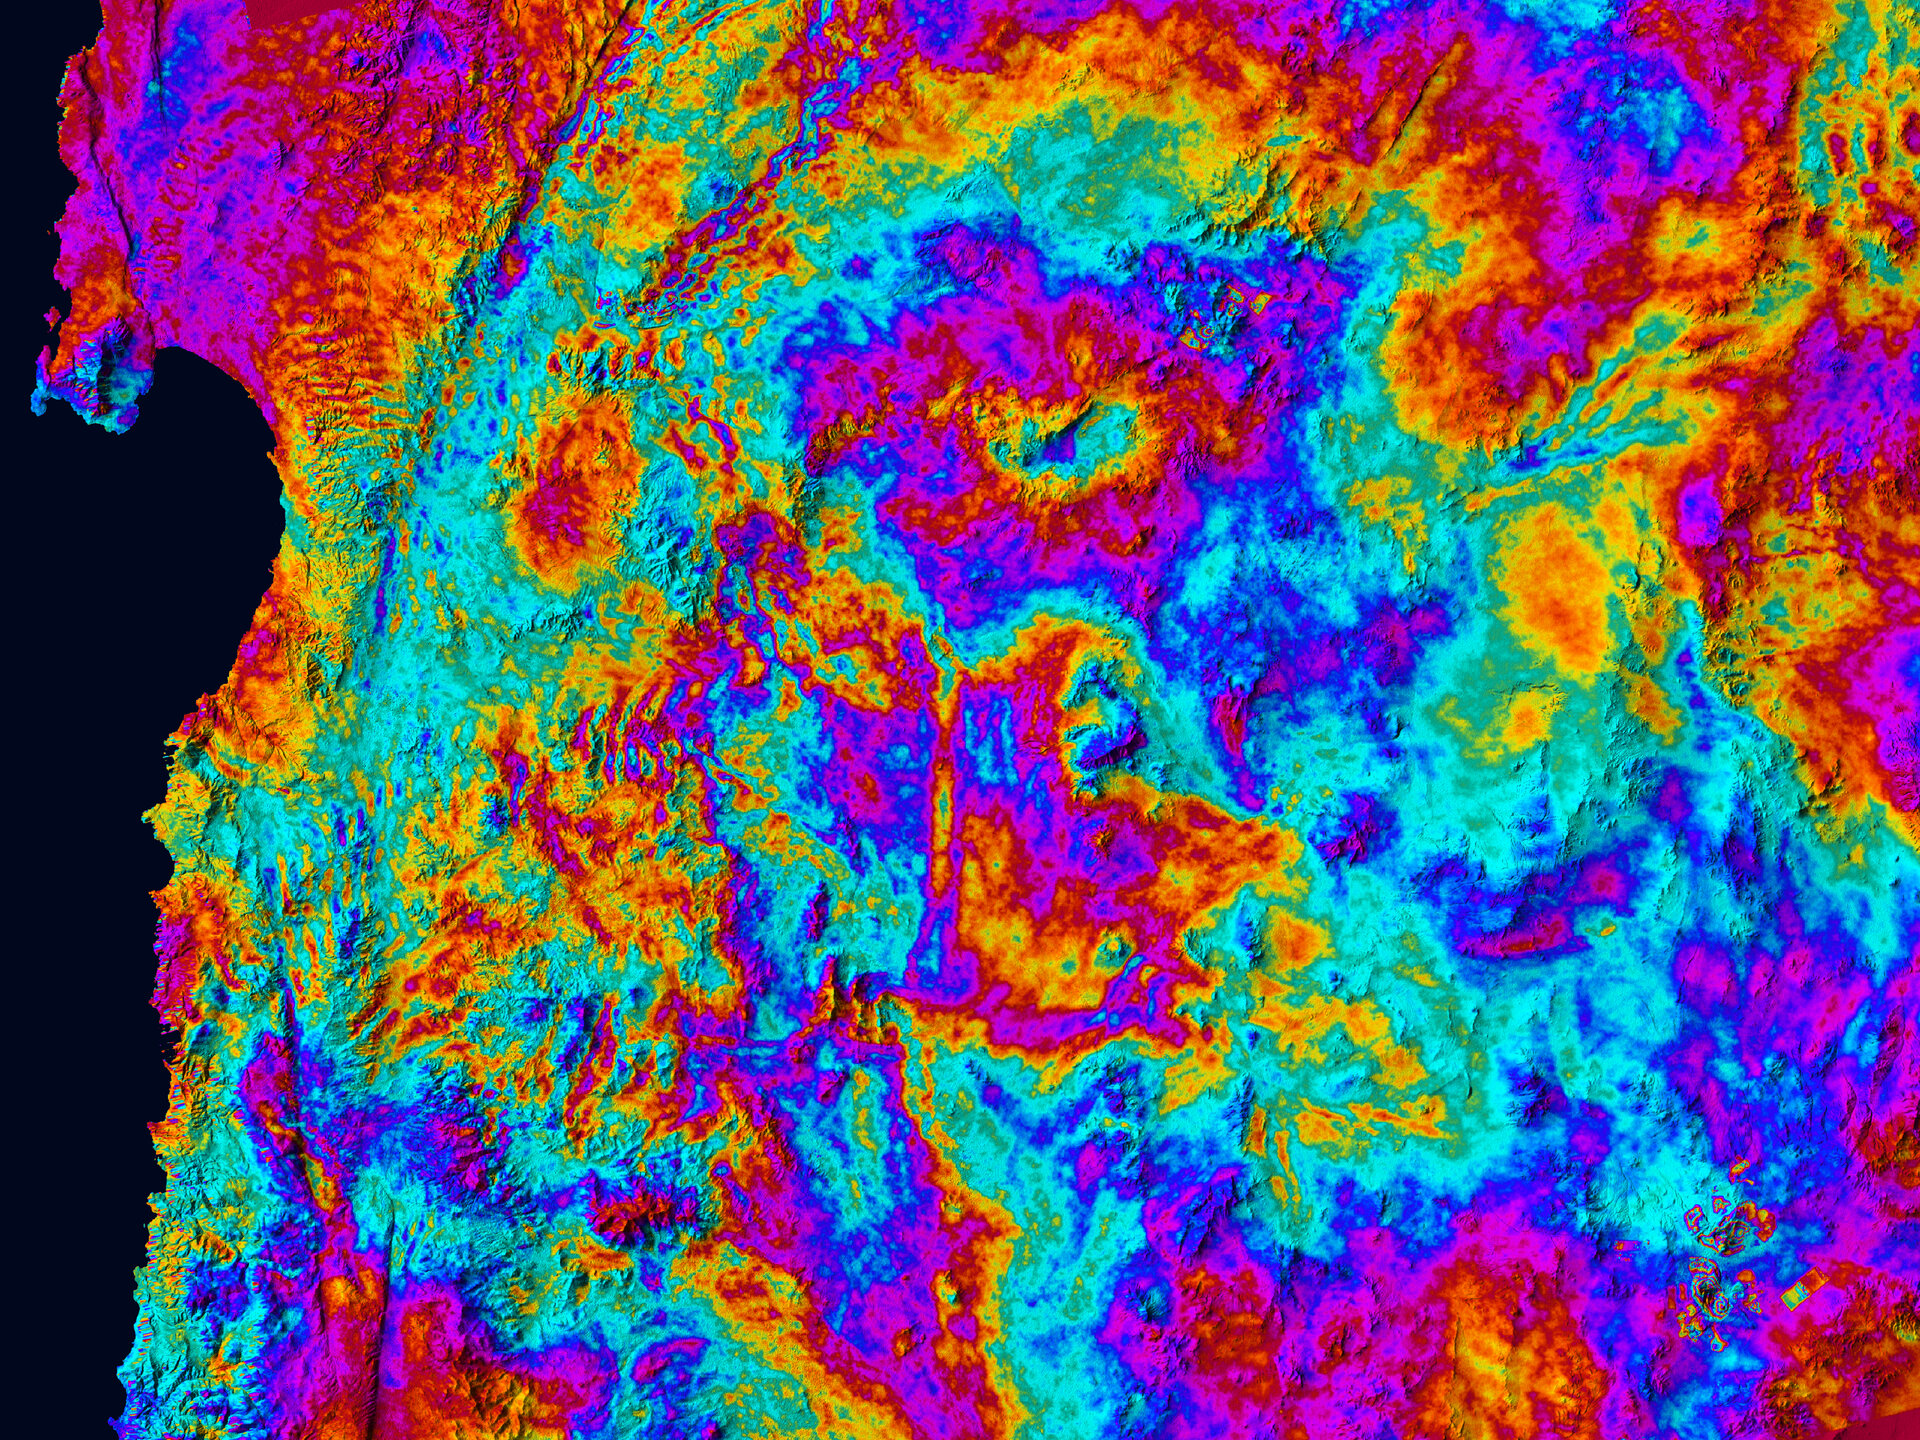
\includegraphics[width=1\linewidth,height=3.64583in]{images/Sentinel-1C_interferogram_of_northern_Chile_pillars.jpg}

}

\caption{Sentinel-1C Interferogram of Northern Chile}

\end{figure}%

\begin{itemize}
\tightlist
\item
  InSAR technique
\item
  Millimeter precision
\item
  Volcano and earthquake monitoring
\end{itemize}

Sentinel-1's ability to penetrate clouds makes it invaluable for flood
mapping during typhoons. The left image shows actual flood monitoring
using Sentinel-1 data. The right image shows an interferogram from
Sentinel-1C demonstrating ground deformation detection with millimeter
precision in northern Chile.

\subsection{Philippine Example: Flood
Monitoring}\label{philippine-example-flood-monitoring}

\begin{center}
\includegraphics[width=0.8\linewidth,height=\textheight,keepaspectratio]{images/sentinel1_flood_ph.png}
\end{center}

\textbf{November 2020: Typhoon Ulysses}

\begin{itemize}
\tightlist
\item
  Extensive flooding in Luzon
\item
  Sentinel-1 detected flood extent
\item
  Rapid mapping capability
\end{itemize}

\textbf{Key Benefits}

\begin{itemize}
\tightlist
\item
  No cloud interference
\item
  Quick response time
\item
  Used for rapid damage assessment
\item
  Supported emergency response
\end{itemize}

During Typhoon Ulysses, Sentinel-1 provided crucial flood extent mapping
when optical satellites couldn't see through clouds. This data supported
PAGASA and NDRRMC response efforts.

\begin{center}\rule{0.5\linewidth}{0.5pt}\end{center}

\section{Sentinel-2: Optical Mission}\label{sentinel-2-optical-mission}

\subsection{Sentinel-2 Overview}\label{sentinel-2-overview}

\textbf{Key Specifications:}

\begin{itemize}
\tightlist
\item
  \textbf{13 spectral bands} (visible, NIR, SWIR)
\item
  \textbf{10m to 60m} spatial resolution
\item
  \textbf{290 km swath} width
\item
  \textbf{5-day revisit} (three satellites operational 2025)
\item
  \textbf{L1C \& L2A} processing levels
\end{itemize}

\textbf{Philippine Example: Mayon Volcano}

\begin{center}
\includegraphics[width=1\linewidth,height=\textheight,keepaspectratio]{images/sentinel2_mayon.jpg}
\end{center}

\textbf{Sentinel-2 monitoring of 2018 eruption}

\begin{itemize}
\tightlist
\item
  False-color composite highlighting lava flows
\item
  10m resolution captures detail
\item
  5-day revisit enables continuous monitoring
\end{itemize}

This Sentinel-2 false-color image of Mayon Volcano from 2018 shows
recent lava flows. With Sentinel-2C operational in 2025, the
three-satellite constellation provides 5-day global revisit.

\subsection{Sentinel-2 Spectral Bands}\label{sentinel-2-spectral-bands}

\begin{longtable}[]{@{}
  >{\raggedright\arraybackslash}p{(\linewidth - 8\tabcolsep) * \real{0.1429}}
  >{\raggedright\arraybackslash}p{(\linewidth - 8\tabcolsep) * \real{0.1429}}
  >{\raggedright\arraybackslash}p{(\linewidth - 8\tabcolsep) * \real{0.3000}}
  >{\raggedright\arraybackslash}p{(\linewidth - 8\tabcolsep) * \real{0.2286}}
  >{\raggedright\arraybackslash}p{(\linewidth - 8\tabcolsep) * \real{0.1857}}@{}}
\toprule\noalign{}
\begin{minipage}[b]{\linewidth}\raggedright
\textbf{Band}
\end{minipage} & \begin{minipage}[b]{\linewidth}\raggedright
\textbf{Name}
\end{minipage} & \begin{minipage}[b]{\linewidth}\raggedright
\textbf{Wavelength (nm)}
\end{minipage} & \begin{minipage}[b]{\linewidth}\raggedright
\textbf{Resolution}
\end{minipage} & \begin{minipage}[b]{\linewidth}\raggedright
\textbf{Purpose}
\end{minipage} \\
\midrule\noalign{}
\endhead
\bottomrule\noalign{}
\endlastfoot
\textbf{B1} & Coastal Aerosol & 443 & 60m & Aerosol correction, water
color \\
\textbf{B2} & Blue & 490 & \textbf{10m} & Water bodies, atmospheric \\
\textbf{B3} & Green & 560 & \textbf{10m} & Vegetation health \\
\textbf{B4} & Red & 665 & \textbf{10m} & Vegetation discrimination \\
\textbf{B5} & Red Edge 1 & 705 & 20m & Vegetation stress detection \\
\textbf{B6} & Red Edge 2 & 740 & 20m & Vegetation classification \\
\textbf{B7} & Red Edge 3 & 783 & 20m & Vegetation stress, chlorophyll \\
\textbf{B8} & NIR & 842 & \textbf{10m} & Biomass, water bodies \\
\textbf{B8A} & NIR Narrow & 865 & 20m & Atmospheric correction \\
\textbf{B9} & Water Vapor & 945 & 60m & Atmospheric correction \\
\textbf{B10} & SWIR Cirrus & 1375 & 60m & Cirrus cloud detection \\
\textbf{B11} & SWIR 1 & 1610 & 20m & Moisture content, fire \\
\textbf{B12} & SWIR 2 & 2190 & 20m & Moisture, geology, soil \\
\end{longtable}

\textbf{All 13 Sentinel-2 bands:} Four 10m bands (B2-B4, B8) for
detailed mapping, six 20m bands including the unique Red Edge trio
(B5-B7) for vegetation analysis, and three 60m atmospheric bands (B1,
B9, B10) for corrections. The Red Edge bands are Sentinel-2's signature
capability.

\subsection{Red Edge Bands - Sentinel-2's Special
Capability}\label{red-edge-bands---sentinel-2s-special-capability}

\textbf{What is Red Edge?}

\begin{itemize}
\tightlist
\item
  Transition zone between red and NIR (700-780nm)
\item
  \textbf{Three dedicated bands (B5, B6, B7)}
\item
  Sensitive to chlorophyll content
\item
  Unique to Sentinel-2 among free satellites
\end{itemize}

\textbf{Applications:}

\begin{itemize}
\tightlist
\item
  Early vegetation stress detection
\item
  Crop health monitoring
\item
  Forest disease identification
\item
  Pre-harvest yield estimation
\end{itemize}

\textbf{Philippine Use Cases:}

\begin{itemize}
\tightlist
\item
  \textbf{Rice crop assessment} - Monitor crop health and nitrogen
  status during panicle initiation in Nueva Ecija rice paddies
\item
  \textbf{Coconut disease detection} - Identify stem bleeding disease
  and pest infestations through spectral signatures
\item
  \textbf{Mangrove health monitoring} - Track vegetation stress and
  recovery in Palawan mangrove forests using red edge indices
\end{itemize}

\emph{Red edge bands detect stress weeks before visible bands show
changes}

Red Edge bands are Sentinel-2's superpower. They detect vegetation
stress weeks before visible bands show changes - crucial for precision
agriculture and forest health monitoring.

\subsection{Sentinel-2 Data Products}\label{sentinel-2-data-products}

\textbf{Level-1C (L1C)}

\begin{itemize}
\tightlist
\item
  Top-of-Atmosphere reflectance
\item
  Radiometrically corrected
\item
  Geometrically refined
\item
  No atmospheric correction
\item
  \textbf{Use:} If you need raw data for custom processing
\end{itemize}

\textbf{Level-2A (L2A)}

\begin{itemize}
\tightlist
\item
  Bottom-of-Atmosphere (surface) reflectance
\item
  Atmospherically corrected
\item
  \textbf{Analysis-ready}
\item
  Scene Classification Layer included
\item
  \textbf{Use:} For most applications - RECOMMENDED
\end{itemize}

\textbf{Always use Level-2A when available - it's analysis-ready!}

L2A data is atmospherically corrected and ready for analysis. Unless you
have a specific reason to use L1C, always choose L2A products.

\subsection{Sentinel-2 Band
Combinations}\label{sentinel-2-band-combinations}

\textbf{True Color (Natural)} - \textbf{RGB:} B4-B3-B2 (Red-Green-Blue)
- Looks like a photograph - Good for visual inspection

\textbf{False Color Infrared} - \textbf{RGB:} B8-B4-B3 (NIR-Red-Green) -
\textbf{Vegetation appears RED} - Classic for vegetation assessment

\textbf{SWIR Composite (Agriculture)} - \textbf{RGB:} B11-B8-B2 -
Highlights crop moisture - Soil moisture visible

\textbf{SWIR-NIR-Red (Burn/Fire)} - \textbf{RGB:} B12-B8-B4 -
\textbf{Active fires appear BRIGHT} - Burn scars dark purple

Different band combinations highlight different features. False Color
(NIR-Red-Green) is the most common for vegetation mapping - healthy
vegetation appears bright red.

\begin{center}\rule{0.5\linewidth}{0.5pt}\end{center}

\section{Sentinel-1 vs Sentinel-2}\label{sentinel-1-vs-sentinel-2}

\subsection{Complementary
Capabilities}\label{complementary-capabilities}

\begin{longtable}[]{@{}
  >{\raggedright\arraybackslash}p{(\linewidth - 4\tabcolsep) * \real{0.2727}}
  >{\raggedright\arraybackslash}p{(\linewidth - 4\tabcolsep) * \real{0.3636}}
  >{\raggedright\arraybackslash}p{(\linewidth - 4\tabcolsep) * \real{0.3636}}@{}}
\toprule\noalign{}
\begin{minipage}[b]{\linewidth}\raggedright
\textbf{Aspect}
\end{minipage} & \begin{minipage}[b]{\linewidth}\raggedright
\textbf{Sentinel-1}
\end{minipage} & \begin{minipage}[b]{\linewidth}\raggedright
\textbf{Sentinel-2}
\end{minipage} \\
\midrule\noalign{}
\endhead
\bottomrule\noalign{}
\endlastfoot
\textbf{Sensor Type} & Radar (SAR) & Optical (MSI) \\
\textbf{Weather} & All-weather & Cloud-affected \\
\textbf{Time} & Day \& night & Daytime only \\
\textbf{Resolution} & 5m × 20m & 10m / 20m / 60m \\
\textbf{Revisit} & 6-12 days & 5 days \\
\textbf{Bands} & Polarizations (2) & Spectral bands (13) \\
\textbf{Best For} & Water, structure, moisture & Vegetation, land cover,
color \\
\end{longtable}

\begin{tcolorbox}[enhanced jigsaw, left=2mm, opacityback=0, toprule=.15mm, breakable, title=\textcolor{quarto-callout-tip-color}{\faLightbulb}\hspace{0.5em}{S1 Flood Mapping Tip}, colbacktitle=quarto-callout-tip-color!10!white, arc=.35mm, titlerule=0mm, colback=white, bottomtitle=1mm, colframe=quarto-callout-tip-color-frame, leftrule=.75mm, toptitle=1mm, rightrule=.15mm, bottomrule=.15mm, opacitybacktitle=0.6, coltitle=black]

\textbf{VV polarization shows dark water} (low backscatter from smooth
surfaces)

\textbf{Best practice:} Compare \textbf{pre-event vs post-event} delta
for reliability

\textbf{Synergy:} Pair S1 (flood extent through clouds) with S2
(vegetation damage when clear) for complete impact assessment

\end{tcolorbox}

Sentinel-1 and Sentinel-2 are complementary. SAR penetrates clouds and
works at night, while optical provides rich spectral information about
surface properties.

\textbf{MICRO-EDIT APPLIED:} Added S1 vs S2 flood tip to set up Day 3
logic - VV dark water, pre/post comparison, and S1+S2 synergy.

\subsection{Synergistic Use Cases}\label{synergistic-use-cases}

\textbf{Flood Mapping}

\begin{itemize}
\tightlist
\item
  \textbf{S1:} Detect water extent (through clouds)
\item
  \textbf{S2:} Assess damage to vegetation/crops (when clear)
\item
  \textbf{Combined:} Complete flood impact assessment
\end{itemize}

\textbf{Forest Monitoring}

\begin{itemize}
\tightlist
\item
  \textbf{S1:} Detect structural changes, biomass
\item
  \textbf{S2:} Identify tree species, health
\item
  \textbf{Combined:} Comprehensive forest mapping
\end{itemize}

\begin{center}
\includegraphics[width=0.6\linewidth,height=\textheight,keepaspectratio]{images/s1_s2_synergy.jpg}
\end{center}

Using both missions together provides more complete information. After a
typhoon, S1 maps floods under clouds while S2 assesses vegetation damage
where it's clear.

\begin{center}\rule{0.5\linewidth}{0.5pt}\end{center}

\subsection{☕ 5-Minute Break}\label{minute-break}

\textbf{Stretch Break}

Stand up • Grab water • Back in 5 minutes

\textbf{Timing:} 5 minutes

\textbf{Instructor Actions:} - Announce break clearly - Mention return
time - Leave slides/browser open for questions - Be available for quick
questions during break

\textbf{When Resuming:} - Wait 1-2 minutes for everyone to return -
Quick recap: ``We've covered Sentinel-1 SAR and Sentinel-2 optical. Now
we'll explore the Philippine EO ecosystem.''

\begin{center}\rule{0.5\linewidth}{0.5pt}\end{center}

\section{Data Access Methods}\label{data-access-methods}

\subsection{Platform Choices for This
Training}\label{platform-choices-for-this-training}

\begin{tcolorbox}[enhanced jigsaw, left=2mm, opacityback=0, toprule=.15mm, breakable, title=\textcolor{quarto-callout-important-color}{\faExclamation}\hspace{0.5em}{Which Platform for Which Task?}, colbacktitle=quarto-callout-important-color!10!white, arc=.35mm, titlerule=0mm, colback=white, bottomtitle=1mm, colframe=quarto-callout-important-color-frame, leftrule=.75mm, toptitle=1mm, rightrule=.15mm, bottomrule=.15mm, opacitybacktitle=0.6, coltitle=black]

Understanding where to work is crucial - don't try to train deep models
on GEE or download 100GB in Colab!

\end{tcolorbox}

\begin{longtable}[]{@{}
  >{\raggedright\arraybackslash}p{(\linewidth - 6\tabcolsep) * \real{0.2041}}
  >{\raggedright\arraybackslash}p{(\linewidth - 6\tabcolsep) * \real{0.2653}}
  >{\raggedright\arraybackslash}p{(\linewidth - 6\tabcolsep) * \real{0.1837}}
  >{\raggedright\arraybackslash}p{(\linewidth - 6\tabcolsep) * \real{0.3469}}@{}}
\toprule\noalign{}
\begin{minipage}[b]{\linewidth}\raggedright
\textbf{Task}
\end{minipage} & \begin{minipage}[b]{\linewidth}\raggedright
\textbf{Platform}
\end{minipage} & \begin{minipage}[b]{\linewidth}\raggedright
\textbf{Why}
\end{minipage} & \begin{minipage}[b]{\linewidth}\raggedright
\textbf{Limitations}
\end{minipage} \\
\midrule\noalign{}
\endhead
\bottomrule\noalign{}
\endlastfoot
\textbf{Data Prep \& Exploration} & \textbf{Google Earth Engine} &
Petabyte catalog, no download, cloud composites & Export limit 32 MB
(tile large areas), no deep learning training \\
\textbf{ML Training (RF, shallow)} & \textbf{GEE or Colab} & RF works in
GEE; small data in Colab & GEE memory limits; Colab free tier quotas \\
\textbf{Deep Learning (CNN, U-Net)} & \textbf{Local GPU / Colab Pro} &
Requires PyTorch/TensorFlow & Colab free = limited GPU time; large
models need local resources \\
\textbf{Large-Scale Processing} & \textbf{CoPhil Mirror Site / COARE} &
400TB local data, HPC resources & Requires account; learning curve for
APIs \\
\textbf{Quick Viz \& Download} & \textbf{Copernicus Browser} &
Interactive, fast previews & Manual selection; bulk downloads tedious \\
\end{longtable}

\textbf{Quotas/Pitfalls to know:} - GEE: Memory errors with large
computations (tile exports!) - Colab Free: GPU disconnects after
inactivity; limited sessions/day - \textbf{CoPhil/Digital Space Campus}:
Hosts this training's materials + local data access

\textbf{P1 IMPROVEMENT APPLIED:} Explicit platform choices table
prevents common mistakes.

\textbf{Key Teaching Points:} - GEE is NOT for training U-Nets or
downloading GBs - Colab free tier has GPU quotas - manage expectations -
CoPhil infrastructure enables local processing - Choose the right tool
for the right job

\textbf{Timing:} 3 minutes

\textbf{Transition:} ``Let's look at these platforms in detail\ldots{}''

\begin{center}\rule{0.5\linewidth}{0.5pt}\end{center}

\subsection{Copernicus Data Space Ecosystem
(2025)}\label{copernicus-data-space-ecosystem-2025}

\begin{center}
\includegraphics[width=0.7\linewidth,height=\textheight,keepaspectratio]{images/dataspace_portal.jpg}
\end{center}

\textbf{New Platform (2023+)}

\begin{itemize}
\tightlist
\item
  Replaced SciHub
\item
  Modern interface
\item
  API access
\item
  Free registration
\end{itemize}

\textbf{Features}

\begin{itemize}
\tightlist
\item
  Search by location/date
\item
  Preview before download
\item
  Direct download
\item
  Bulk processing
\end{itemize}

\textbf{URL:} \url{https://dataspace.copernicus.eu}

The Copernicus Data Space Ecosystem is the new portal replacing the
legacy SciHub. All Sentinel data are free and open.

\subsection{SentiBoard Dashboard (October
2025)}\label{sentiboard-dashboard-october-2025}

\begin{center}
\includegraphics[width=0.75\linewidth,height=\textheight,keepaspectratio]{images/sentiboard.jpg}
\end{center}

\begin{itemize}
\tightlist
\item
  \textbf{Real-time mission status}
\item
  Data availability insights
\item
  Acquisition plans
\item
  Quality metrics
\item
  Interactive dashboard
\end{itemize}

SentiBoard is a new feature (October 2025) providing real-time insights
into Copernicus Sentinel missions and data availability.

\subsection{Google Earth Engine}\label{google-earth-engine}

\textbf{Planetary-Scale Platform}

\begin{itemize}
\tightlist
\item
  Petabyte-scale data catalog
\item
  All Sentinel-1 \& Sentinel-2 data
\item
  Cloud-based processing
\item
  Free for research/education
\item
  \textbf{No download needed!}
\end{itemize}

\includegraphics[width=1\linewidth,height=\textheight,keepaspectratio]{images/gee_logo.png}

\textbf{We'll use GEE extensively in this training}

\textbf{URL:} \url{https://earthengine.google.com}

Google Earth Engine provides ready access to all Sentinel data with
cloud-based processing. We'll use GEE extensively for data access and
preprocessing.

\subsection{Alternative Data Sources}\label{alternative-data-sources}

\textbf{Alaska Satellite Facility (ASF)}

\begin{itemize}
\tightlist
\item
  Sentinel-1 specialist
\item
  User-friendly interface
\item
  Preprocessing tools
\item
  \url{https://asf.alaska.edu}
\end{itemize}

\textbf{AWS Open Data}

\begin{itemize}
\tightlist
\item
  Sentinel-2 on AWS
\item
  Cloud-optimized
\item
  Pay for compute only
\item
  Programmatic access
\end{itemize}

\textbf{Now Available: CoPhil Mirror Site in the Philippines!}
(Operational 2024-2025)

\textbf{MICRO-EDIT APPLIED:} Mirror Site is NOW operational (not
``coming soon'').

Multiple platforms provide Sentinel data access. The CoPhil Mirror Site
provides \textbf{local data access in the Philippines for faster
downloads} - critical for reducing international bandwidth bottlenecks.

\textbf{Key Point:} 400TB capacity, focused on PH scenes, free for
government/academia/researchers

\section{Part 2: Philippine EO
Ecosystem}\label{part-2-philippine-eo-ecosystem}

\subsection{Overview of Philippine EO
Landscape}\label{overview-of-philippine-eo-landscape}

\begin{center}
\includegraphics[width=0.85\linewidth,height=\textheight,keepaspectratio]{images/ph_eo_ecosystem.png}
\end{center}

\begin{itemize}
\tightlist
\item
  \textbf{PhilSA:} Space data and operations
\item
  \textbf{NAMRIA:} National mapping and geospatial data
\item
  \textbf{DOST-ASTI:} AI and remote sensing R\&D
\item
  \textbf{PAGASA:} Climate and weather data
\end{itemize}

Beyond European satellites, the Philippines has its own geospatial data
platforms and agencies that provide crucial complementary data and
support.

\section{Philippine Space Agency
(PhilSA)}\label{philippine-space-agency-philsa}

\subsection{PhilSA: National Space
Agency}\label{philsa-national-space-agency}

\textbf{Established:} August 2019

\textbf{Mandate:}

\begin{itemize}
\tightlist
\item
  Central civilian space agency
\item
  Promote space data use
\item
  Build national capacity
\item
  Support DRR, CCA, NRM
\item
  Co-chair CoPhil programme
\end{itemize}

\includegraphics[width=1\linewidth,height=\textheight,keepaspectratio]{images/philsa_building.jpg}

\textbf{Website:} \url{https://philsa.gov.ph}

PhilSA is the central civilian space agency established in 2019. As
co-chair of CoPhil, PhilSA is leading national efforts to leverage
Copernicus data.

\subsection{SIYASAT Data Portal}\label{siyasat-data-portal}

\begin{center}
\includegraphics[width=0.7\linewidth,height=\textheight,keepaspectratio]{images/siyasat_portal.jpg}
\end{center}

\textbf{Purpose (2025)}

\begin{itemize}
\tightlist
\item
  Secure data archive \textbf{operational}
\item
  Visualization system
\item
  Data distribution
\item
  Maritime \& terrestrial monitoring
\end{itemize}

\textbf{Data Types}

\begin{itemize}
\tightlist
\item
  NovaSAR-1 radar imagery
\item
  AIS ship tracking data
\item
  Processed products
\item
  Analysis-ready data
\end{itemize}

\textbf{Timing:} 3 minutes

\textbf{Key Points:} - SIYASAT (Secure Interactive Yield-Assessment \&
SAR Analytics Tools) is PhilSA's operational data portal - \textbf{2025
Status:} Fully operational with NovaSAR-1 data access - Provides secure
archive for Philippine government agencies - Critical for maritime
security (illegal fishing, territorial monitoring) - Registration
required - priority for government agencies

\textbf{Transition:} ``Beyond PhilSA, DOST-ASTI is leading AI innovation
for EO applications\ldots{}''

\subsection{Space+ Data Dashboard}\label{space-data-dashboard}

\begin{center}
\includegraphics[width=0.75\linewidth,height=\textheight,keepaspectratio]{images/space_plus_dashboard.jpg}
\end{center}

\begin{itemize}
\tightlist
\item
  \textbf{User-friendly web portal}
\item
  Browse satellite imagery
\item
  Visualization tools
\item
  Download datasets
\item
  \textbf{No programming required}
\item
  Open to government, researchers, public
\end{itemize}

The Space+ Data Dashboard democratizes access to satellite data, making
it available to local governments, researchers, and even students
without requiring programming skills.

\subsection{PhilSA 2025 Initiatives}\label{philsa-2025-initiatives}

\textbf{Space Business Innovation Challenge}

\begin{itemize}
\tightlist
\item
  Empowers Filipino innovators
\item
  Free satellite data access
\item
  Build solutions for local needs
\item
  Earth observation focus
\item
  Weather \& environmental data
\end{itemize}

\textbf{Training Programs}

\begin{itemize}
\tightlist
\item
  Downstream data utilization
\item
  Practical applications
\item
  Capacity building nationwide
\item
  Partnership with DOST
\end{itemize}

PhilSA's 2025 initiatives focus on empowering innovators and building
capacity across the Philippines to use satellite data effectively.

\subsection{COARE Infrastructure}\label{coare-infrastructure}

\textbf{Computing and Archiving Research Environment}

\begin{itemize}
\tightlist
\item
  High-performance computing
\item
  Data archiving capabilities
\item
  Science cloud facilities
\item
  Supports data-intensive research
\item
  Enables AI/ML workflows
\end{itemize}

\includegraphics[width=1\linewidth,height=\textheight,keepaspectratio]{images/coare_infrastructure.jpg}

COARE provides the computational infrastructure needed for processing
large satellite datasets and running AI/ML models at scale.

\section{NAMRIA}\label{namria}

\subsection{NAMRIA: National Mapping
Authority}\label{namria-national-mapping-authority}

\textbf{National Mapping and Resource Information Authority}

\textbf{Role:}

\begin{itemize}
\tightlist
\item
  Official mapping agency
\item
  Authoritative geospatial data
\item
  Topographic maps
\item
  Hazard maps
\item
  Land cover datasets
\end{itemize}

\includegraphics[width=1.5625in,height=\textheight,keepaspectratio]{images/namria_logo.png}

\textbf{Website:} \url{https://www.geoportal.gov.ph}

NAMRIA is the national mapping agency responsible for topographic maps,
hydrographic data, and authoritative geospatial datasets.

\subsection{NAMRIA Geoportal}\label{namria-geoportal}

\begin{center}
\includegraphics[width=0.75\linewidth,height=\textheight,keepaspectratio]{images/namria_geoportal.jpg}
\end{center}

\textbf{One-Stop Shop for Philippine Geospatial Data}

\begin{itemize}
\tightlist
\item
  National basemaps (1:50,000 scale)
\item
  Administrative boundaries
\item
  Topographic maps
\item
  Thematic maps
\item
  \textbf{Downloadable shapefiles and rasters}
\end{itemize}

The NAMRIA Geoportal is the go-to source for official Philippine spatial
data including boundaries, topographic maps, and land cover data.

\subsection{Land Cover Mapping
Project}\label{land-cover-mapping-project}

\begin{center}
\includegraphics[width=0.7\linewidth,height=\textheight,keepaspectratio]{images/namria_landcover.jpg}
\end{center}

\textbf{Latest:} 2020 National Land Cover

\textbf{Classes:}

\begin{itemize}
\tightlist
\item
  Forest types
\item
  Agriculture
\item
  Built-up areas
\item
  Water bodies
\item
  Wetlands
\item
  Barren land
\end{itemize}

\textbf{Data Formats:}

\begin{itemize}
\tightlist
\item
  Shapefile
\item
  GeoTIFF
\item
  CSV
\item
  GeoJSON
\item
  KML
\item
  PNG
\end{itemize}

\textbf{Portal:}
\url{https://land-cover-mapping-project-namria.hub.arcgis.com}

NAMRIA's land cover datasets are valuable for validation and comparison
with satellite-derived classifications. The 2020 national land cover map
is available in multiple formats.

\subsection{HazardHunterPH Portal}\label{hazardhunterph-portal}

\begin{center}
\includegraphics[width=0.75\linewidth,height=\textheight,keepaspectratio]{images/hazardhunter.jpg}
\end{center}

\textbf{Comprehensive Hazard Assessment Platform}

\textbf{Hazard Types:}

\begin{itemize}
\tightlist
\item
  Earthquake-induced hazards
\item
  Active fault lines
\item
  Tsunami susceptibility
\item
  Liquefaction zones
\item
  Landslide hazards
\end{itemize}

\textbf{Applications:}

\begin{itemize}
\tightlist
\item
  Disaster risk assessment
\item
  Land use planning
\item
  Infrastructure siting
\item
  Emergency preparedness
\end{itemize}

\textbf{URL:} \url{https://hazardhunter.georisk.gov.ph/map}

HazardHunterPH provides critical hazard data for DRR planning. These
maps can be overlaid with satellite data for vulnerability assessments.

\subsection{How NAMRIA Complements Sentinel
Data}\label{how-namria-complements-sentinel-data}

\textbf{Sentinel Imagery Provides:}

\begin{itemize}
\tightlist
\item
  Current conditions
\item
  Frequent updates
\item
  Large-area coverage
\item
  Multi-temporal analysis
\end{itemize}

\textbf{NAMRIA Data Provides:}

\begin{itemize}
\tightlist
\item
  \textbf{Ground truth for validation}
\item
  \textbf{Training labels for ML models}
\item
  Historical baselines
\item
  Official classifications
\item
  Hazard context
\end{itemize}

\begin{tcolorbox}[enhanced jigsaw, left=2mm, opacityback=0, toprule=.15mm, breakable, title=\textcolor{quarto-callout-tip-color}{\faLightbulb}\hspace{0.5em}{MICRO-EDIT: Using NAMRIA/Space+ as Label Sources}, colbacktitle=quarto-callout-tip-color!10!white, arc=.35mm, titlerule=0mm, colback=white, bottomtitle=1mm, colframe=quarto-callout-tip-color-frame, leftrule=.75mm, toptitle=1mm, rightrule=.15mm, bottomrule=.15mm, opacitybacktitle=0.6, coltitle=black]

\textbf{For Day 2 Palawan RF lab:} 1. Download NAMRIA land cover
shapefile (authoritative classes) 2. Overlay on Sentinel-2 imagery 3.
Extract training points per class (forest, agriculture, water, etc.) 4.
Train Random Forest classifier 5. Validate predictions against NAMRIA
hold-out samples

\textbf{Space+ Dashboard} also provides admin boundaries and
infrastructure layers for context in all visualizations.

\end{tcolorbox}

\textbf{Example:} Use Sentinel-2 to map current land cover, validate
against NAMRIA's official 2020 map, detect changes

\textbf{MICRO-EDIT APPLIED:} Explicit link between NAMRIA/Space+ as
\textbf{label sources \& validation layers}, not just context.

NAMRIA data provides essential ground truth and context for
satellite-based analysis. Official boundaries and hazard maps enhance
satellite data interpretation.

\textbf{Show one example overlay:} NAMRIA training polygons (land cover
classes) overlaid on S2 RGB composite.

\section{DOST-ASTI AI Initiatives}\label{dost-asti-ai-initiatives}

\subsection{DOST-ASTI Overview}\label{dost-asti-overview}

\textbf{Advanced Science and Technology Institute}

\begin{itemize}
\tightlist
\item
  Lead agency for EO and AI R\&D
\item
  Remote sensing expertise
\item
  Machine learning development
\item
  National AI infrastructure
\item
  \textbf{P2.6 billion investment until 2028}
\end{itemize}

\includegraphics[width=1.5625in,height=\textheight,keepaspectratio]{images/dost_asti_logo.png}

\textbf{Website:} \url{https://asti.dost.gov.ph}

DOST-ASTI leads several projects at the intersection of remote sensing,
AI, and big data, with significant national investment of P2.6 billion
through 2028.

\subsection{DATOS: Remote Sensing Help
Desk}\label{datos-remote-sensing-help-desk}

\begin{center}
\includegraphics[width=0.4\linewidth,height=\textheight,keepaspectratio]{images/datos_logo.png}
\end{center}

\begin{itemize}
\tightlist
\item
  \textbf{Remote Sensing and Data Science Help Desk}
\item
  Rapid analytics during disasters
\item
  Flood mapping from satellite imagery
\item
  Damage assessment
\item
  Crop mapping (rice, sugarcane)
\item
  Road network detection
\item
  Supports emergency response agencies
\end{itemize}

During past typhoons, DATOS used satellite images to produce flood maps
and give them to disaster response agencies within hours. They also
worked on crop mapping and infrastructure detection using AI.

\subsection{SkAI-Pinas Programme}\label{skai-pinas-programme}

\begin{center}
\includegraphics[width=0.75\linewidth,height=\textheight,keepaspectratio]{images/skai_pinas.jpg}
\end{center}

\textbf{Philippine Sky AI Program (2021-2028)}

\begin{itemize}
\tightlist
\item
  Flagship AI R\&D programme
\item
  \textbf{Part of P2.6B DOST AI investment}
\item
  Democratize AI across Philippines
\item
  Remote sensing \& big data focus
\end{itemize}

\textbf{Impact (2025)}

\begin{itemize}
\tightlist
\item
  300+ institutions supported
\item
  Universities \& colleges
\item
  SMEs \& research teams
\item
  Local government units
\end{itemize}

\textbf{Timing:} 3 minutes

\textbf{Key Points:} - \textbf{2025 Update:} SkAI-Pinas is part of
DOST's P2.6 billion AI investment (2024-2028) - Focuses on democratizing
AI for EO applications - Provides infrastructure, training, and support
- Successfully engaged 300+ institutions nationwide - Critical for
building national AI capacity

\textbf{Examples:} - Universities using SkAI for flood mapping research
- LGUs leveraging AI for disaster preparedness - SMEs building EO-based
agricultural solutions

\textbf{Transition:} ``SkAI provides the platform. DIMER provides the
models. PANDA brings it all together\ldots{}''

\subsection{DIMER: AI Model Hub}\label{dimer-ai-model-hub}

\begin{center}
\includegraphics[width=0.7\linewidth,height=\textheight,keepaspectratio]{images/dimer_interface.jpg}
\end{center}

\textbf{Democratized Intelligent Model Exchange Repository}

\begin{itemize}
\tightlist
\item
  Digital ``model store''
\item
  Pre-trained AI models
\item
  Ready-to-use
\item
  Filipino-specific challenges
\end{itemize}

\textbf{Available Models}

\begin{itemize}
\tightlist
\item
  Landslide detection
\item
  Traffic surveys
\item
  Crop monitoring
\item
  Land cover classification
\item
  Flood detection
\end{itemize}

DIMER lowers barriers to AI by enabling end-users to reuse optimized AI
models. If you need a model for land cover or flood detection, check
DIMER first before building from scratch.

\subsection{AIPI: AI Processing
Interface}\label{aipi-ai-processing-interface}

\textbf{Purpose}

\begin{itemize}
\tightlist
\item
  Streamline large-scale remote sensing tasks
\item
  Reduce computational barriers
\item
  Run AI models on ASTI servers
\item
  Process hundreds of images efficiently
\end{itemize}

\includegraphics[width=1\linewidth,height=\textheight,keepaspectratio]{images/aipi_workflow.png}

\textbf{Example:} Apply an AI model to 100 Sentinel-2 images over entire
region without your laptop

AIPI allows users to run large computations on ASTI's servers without
heavy local processing. This is especially valuable when processing many
satellite images with AI models.

\subsection{ALaM: Automated Labeling
Machine}\label{alam-automated-labeling-machine}

\textbf{Challenge}

Creating labeled training data is:

\begin{itemize}
\tightlist
\item
  Time-consuming
\item
  Expensive
\item
  Requires expertise
\item
  Major bottleneck for AI
\end{itemize}

\textbf{ALaM Solution}

\begin{itemize}
\tightlist
\item
  Automate labeling process
\item
  Crowdsourcing capabilities
\item
  Expert validation
\item
  Build training datasets
\end{itemize}

\textbf{Result:} Faster creation of high-quality training data for
Filipino contexts

Creating labeled data is a big challenge in EO AI. ALaM tries to address
this through automation and crowdsourcing, making it easier to build
training datasets for Philippine applications.

\subsection{How DOST-ASTI Tools Work
Together}\label{how-dost-asti-tools-work-together}

\begin{center}
\includegraphics[width=0.8\linewidth,height=\textheight,keepaspectratio]{images/asti_ecosystem.png}
\end{center}

\begin{enumerate}
\def\labelenumi{\arabic{enumi}.}
\tightlist
\item
  \textbf{ALaM} creates training data
\item
  Train models and share via \textbf{DIMER}
\item
  Process large datasets with \textbf{AIPI}
\item
  Deploy for operational use via \textbf{SkAI-Pinas}
\item
  Support disaster response through \textbf{DATOS}
\end{enumerate}

These initiatives work together to create a complete ecosystem from data
labeling through model development to operational deployment.

\section{PAGASA \& Other Data Sources}\label{pagasa-other-data-sources}

\subsection{PAGASA: Weather \& Climate
Data}\label{pagasa-weather-climate-data}

\textbf{Philippine Atmospheric, Geophysical and Astronomical Services
Administration}

\textbf{Data Types:}

\begin{itemize}
\tightlist
\item
  Historical rainfall
\item
  Temperature records
\item
  Typhoon tracks
\item
  Climate forecasts
\item
  Weather observations
\end{itemize}

\includegraphics[width=1.5625in,height=\textheight,keepaspectratio]{images/pagasa_logo.png}

\textbf{Integration:} Combine with satellite data for climate analysis

PAGASA provides meteorological and climate data that can be integrated
with satellite observations for comprehensive analysis. Rainfall data +
flood maps, for example.

\subsection{Synergy: Satellite + Ground
Data}\label{synergy-satellite-ground-data}

\textbf{Satellite Data (Sentinel)}

\begin{itemize}
\tightlist
\item
  Spatial coverage
\item
  Consistent acquisition
\item
  Multiple variables
\item
  Time series
\end{itemize}

\textbf{Ground Data (Philippine agencies)}

\begin{itemize}
\tightlist
\item
  Point validation
\item
  Ground truth
\item
  Meteorological context
\item
  Local expertise
\end{itemize}

\textbf{Combined = More robust analysis and higher confidence}

The Philippines is developing a rich EO ecosystem. The goal of CoPhil is
to ensure you can leverage both international (Sentinel) and national
data together effectively.

\section{CoPhil Infrastructure}\label{cophil-infrastructure}

\subsection{CoPhil Mirror Site}\label{cophil-mirror-site}

\begin{center}
\includegraphics[width=0.7\linewidth,height=\textheight,keepaspectratio]{images/mirror_site_concept.jpg}
\end{center}

\begin{itemize}
\tightlist
\item
  \textbf{Philippines-based Copernicus data repository}
\item
  Local mirror of Sentinel data
\item
  Focus on Philippine region
\item
  Faster access (no international bandwidth)
\item
  Reliable availability
\item
  \textbf{Operational by 2025}
\item
  Hosted by PhilSA with CloudFerro support
\end{itemize}

The CoPhil Mirror Site will locally store Sentinel data focused on the
Philippines, enabling much faster downloads than from European servers.

\subsection{Digital Space Campus}\label{digital-space-campus}

\begin{center}
\includegraphics[width=0.75\linewidth,height=\textheight,keepaspectratio]{images/digital_campus.jpg}
\end{center}

\textbf{Purpose}

\begin{itemize}
\tightlist
\item
  Online learning portal
\item
  Training materials repository
\item
  Self-paced learning
\item
  Community of practice
\item
  Knowledge sharing
\end{itemize}

\textbf{Content}

\begin{itemize}
\tightlist
\item
  Course presentations
\item
  Jupyter notebooks
\item
  Datasets
\item
  Guides \& tutorials
\item
  Forum discussions
\end{itemize}

All materials from this 4-day training will be available on the Digital
Space Campus for future reference and for colleagues who couldn't
attend.

\subsection{Building a Sustainable EO
Ecosystem}\label{building-a-sustainable-eo-ecosystem}

\begin{enumerate}
\def\labelenumi{\arabic{enumi}.}
\tightlist
\item
  \textbf{Data Access:} Mirror Site + Data Space Ecosystem
\item
  \textbf{Processing:} COARE + AIPI + Google Earth Engine
\item
  \textbf{Models:} DIMER repository
\item
  \textbf{Training:} Digital Space Campus
\item
  \textbf{Operations:} DATOS + Agency integration
\item
  \textbf{Community:} SkAI-Pinas network
\end{enumerate}

\textbf{Result:} Complete infrastructure for operational EO AI/ML**

CoPhil is building sustainable infrastructure ensuring you can continue
working with Sentinel data and AI/ML tools after this training, without
starting from scratch.

\section{Summary \& Integration}\label{summary-integration}

\subsection{Key Takeaways}\label{key-takeaways}

\begin{enumerate}
\def\labelenumi{\arabic{enumi}.}
\tightlist
\item
  \textbf{Copernicus} provides free, high-quality satellite data
  globally
\item
  \textbf{Sentinel-1} (SAR) works day/night, all-weather - essential for
  tropics
\item
  \textbf{Sentinel-2} (optical) provides rich spectral information - 5
  day revisit
\item
  \textbf{Multiple access methods} available (Data Space, GEE, Mirror
  Site)
\item
  \textbf{Philippine agencies} provide complementary data and expertise
\item
  \textbf{CoPhil infrastructure} supports sustainable capacity building
\end{enumerate}

You now understand the full picture from data sources through national
infrastructure. This foundation supports all subsequent AI/ML work.

\subsection{How It All Connects}\label{how-it-all-connects}

\begin{center}
\includegraphics[width=0.9\linewidth,height=\textheight,keepaspectratio]{images/integration_diagram.png}
\end{center}

Satellite data + Philippine ground truth + AI models + processing
infrastructure = Operational applications for DRR, CCA, and NRM

\subsection{Example Workflow: Flood
Mapping}\label{example-workflow-flood-mapping}

\begin{enumerate}
\def\labelenumi{\arabic{enumi}.}
\tightlist
\item
  \textbf{Acquire} Sentinel-1 SAR data (GEE or Mirror Site)
\item
  \textbf{Validate} with PAGASA rainfall data
\item
  \textbf{Process} using AI model from DIMER
\item
  \textbf{Scale} processing via AIPI
\item
  \textbf{Combine} with NAMRIA hazard maps
\item
  \textbf{Deliver} to NDRRMC via DATOS
\end{enumerate}

\textbf{This is what integrated EO capacity looks like!}

A real-world workflow leverages multiple data sources, AI tools, and
institutional partnerships. This is exactly what CoPhil aims to enable.

\begin{center}\rule{0.5\linewidth}{0.5pt}\end{center}

\subsection{Operational Cautions}\label{operational-cautions}

\begin{tcolorbox}[enhanced jigsaw, left=2mm, opacityback=0, toprule=.15mm, breakable, title=\textcolor{quarto-callout-warning-color}{\faExclamationTriangle}\hspace{0.5em}{``Don't Do This'' - Common Pitfalls}, colbacktitle=quarto-callout-warning-color!10!white, arc=.35mm, titlerule=0mm, colback=white, bottomtitle=1mm, colframe=quarto-callout-warning-color-frame, leftrule=.75mm, toptitle=1mm, rightrule=.15mm, bottomrule=.15mm, opacitybacktitle=0.6, coltitle=black]

\textbf{Quality \& Governance additions} to prevent common mistakes:

\end{tcolorbox}

\textbf{Model Applicability:} - ❌ \textbf{Don't} apply a Palawan RF
land cover model to Mindanao without re-sampling - Why: Different
climate, vegetation types, seasonality - Do: Collect local training
samples from Mindanao - ❌ \textbf{Don't} use un-calibrated SAR (digital
numbers only) - Why: Meaningless for quantitative analysis - Do: Always
calibrate to σ⁰ or γ⁰ in dB

\textbf{Processing Assumptions:} - ❌ \textbf{Don't} skip terrain
correction (RTC) for SAR in mountainous areas - Why: Topographic
distortions create false changes - Do: Apply RTC using SRTM or better
DEM - ❌ \textbf{Don't} mix Sentinel-2 processing baselines without
harmonization - Why: DN offset of 1000 after Jan 2022 breaks time series
- Do: Use HARMONIZED collections in GEE

\textbf{Evaluation:} - ❌ \textbf{Don't} train and test on the same
tile/province - Why: Inflated accuracy, poor generalization - Do:
Geographic hold-out (different tiles/provinces for test)

\textbf{P2 IMPROVEMENT APPLIED:} Operational cautions slide with ``don't
do this'' examples.

These are real mistakes participants WILL make without explicit
warnings. One slide can save hours of debugging and poor results.

\begin{center}\rule{0.5\linewidth}{0.5pt}\end{center}

\subsection{Pre-Flight Checklist}\label{pre-flight-checklist}

\begin{tcolorbox}[enhanced jigsaw, left=2mm, opacityback=0, toprule=.15mm, breakable, title=\textcolor{quarto-callout-note-color}{\faInfo}\hspace{0.5em}{P1 IMPROVEMENT: Before Day 1 Hands-On Sessions}, colbacktitle=quarto-callout-note-color!10!white, arc=.35mm, titlerule=0mm, colback=white, bottomtitle=1mm, colframe=quarto-callout-note-color-frame, leftrule=.75mm, toptitle=1mm, rightrule=.15mm, bottomrule=.15mm, opacitybacktitle=0.6, coltitle=black]

\textbf{Send this checklist 1 week before training:}

\end{tcolorbox}

\textbf{✅ Accounts \& Access:} - {[} {]} Google Earth Engine account
enabled
(\href{https://signup.earthengine.google.com}{signup.earthengine.google.com})
- {[} {]} Google Drive with ≥5 GB free space - {[} {]} Google Colab
tested (login with same Google account) - {[} {]} CoPhil Infrastructure
registration
(\href{https://application.infra.copphil.philsa.gov.ph}{application.infra.copphil.philsa.gov.ph})

\textbf{✅ Software \& Data:} - {[} {]} Downloaded sample vector/raster
bundle (link provided via email) - {[} {]} Confirmed zip file extracts
correctly - {[} {]} Python 3.8+ installed (if working locally) - {[} {]}
Jupyter notebook tested (if working locally)

\textbf{✅ Troubleshooting Contacts:} - {[} {]} Have training support
email/chat details - {[} {]} Know how to access Digital Space Campus
materials

\textbf{If any issues:} Contact training organizers BEFORE Day 1 to
resolve access problems!

\textbf{P1 IMPROVEMENT APPLIED:} Pre-flight checklist (send 1 week
before).

\textbf{Action Item for Organizers:} - Create downloadable ``sample
bundle'' (small GeoPackage + COG) - Set up support email/chat channel -
Send checklist email 7 days before training - Follow up 2 days before to
confirm readiness

\begin{center}\rule{0.5\linewidth}{0.5pt}\end{center}

\subsection{What's Next in Day 1?}\label{whats-next-in-day-1}

\textbf{Session 2 (Next)}

\begin{itemize}
\tightlist
\item
  AI/ML fundamentals
\item
  Supervised vs unsupervised learning
\item
  Neural networks basics
\item
  Data-centric AI
\item
  \textbf{→ 5-min Concept Check} (3 questions)
\end{itemize}

\textbf{Sessions 3 \& 4}

\begin{itemize}
\tightlist
\item
  Hands-on Python (GeoPandas, Rasterio)

  \begin{itemize}
  \tightlist
  \item
    \textbf{Pre-run pip installs} to save time
  \end{itemize}
\item
  Google Earth Engine tutorial

  \begin{itemize}
  \tightlist
  \item
    \textbf{Start from ready script}, modify filters only
  \end{itemize}
\item
  Access real Sentinel data
\item
  \textbf{SCL cloud/shadow masking} (not QA60)
\end{itemize}

Now that you understand where data comes from, we'll learn how AI/ML can
extract information from these data, then get hands-on with actual
satellite imagery.

\textbf{P1 IMPROVEMENTS NOTED:} - Concept check after Session 2 -
Pre-run installations in Session 3 - Ready GEE script in Session 4
(modify filters live, don't type from scratch)

\subsection{Session Summary}\label{session-summary}

\textbf{What We Covered:}

✅ Copernicus Programme \& free/open data policy\\
✅ Sentinel-1 (SAR) - all-weather monitoring\\
✅ Sentinel-2 (Optical) - 13 bands, 10m resolution\\
✅ \textbf{2025 Updates:} 1C \& 2C operational\\
✅ Philippine EO infrastructure (PhilSA, NAMRIA, DOST-ASTI)\\
✅ Data access platforms (SIYASAT, Geoportal, SkAI-Pinas)

\textbf{Timing:} 2 minutes

\textbf{Key Takeaways:} - You now understand WHERE EO data comes from -
You know WHAT satellites provide what data - You know HOW to access data
(both EU and PH platforms) - Ready for Session 2: Learning WHAT to do
with this data using AI/ML

\begin{center}\rule{0.5\linewidth}{0.5pt}\end{center}

\subsection{Q\&A}\label{qa}

\textbf{Copernicus \& Sentinel}

\begin{itemize}
\tightlist
\item
  Mission specifications?
\item
  Data products \& formats?
\item
  Access methods?
\item
  Processing levels?
\end{itemize}

\textbf{Philippine EO Ecosystem}

\begin{itemize}
\tightlist
\item
  Agency roles \& mandates?
\item
  Data access procedures?
\item
  Integration with Copernicus?
\item
  P2.6B AI investment details?
\end{itemize}

\textbf{Timing:} 3-5 minutes for Q\&A

\textbf{Facilitation Tips:} - Encourage questions from different agency
participants - Share knowledge across government, academic, private
sectors - If technical question about access, note for Session 4 (GEE
hands-on) - Keep responses brief - detailed hands-on coming in Sessions
3-4

\textbf{Common Questions \& Answers:} - ``How do I sign up for GEE?'' →
Will cover in Session 4 - ``Which satellite should I use?'' → Depends on
application (Day 2 topic) - ``Is SIYASAT public?'' → Registration
required, priority for gov agencies - ``Can I combine Sentinel-1 and
-2?'' → Yes! Synergistic use cases discussed today

\section{Next: Session 2}\label{next-session-2}

\subsection{Core Concepts of AI/ML for Earth
Observation}\label{core-concepts-of-aiml-for-earth-observation}

\textbf{Coming up after break:}

\begin{itemize}
\tightlist
\item
  What is AI/ML and why for EO?
\item
  The EO AI/ML workflow
\item
  Supervised vs unsupervised learning
\item
  Introduction to deep learning
\item
  Data-centric AI approaches
\end{itemize}

\textbf{See you in Session 2! 🚀}

\begin{center}\rule{0.5\linewidth}{0.5pt}\end{center}

\section{Thank You!}\label{thank-you}

\subsection{Contact \& Resources}\label{contact-resources}

\textbf{European Platforms:}\\
Copernicus Data Space: \url{https://dataspace.copernicus.eu}\\
CoPhil Programme: \url{https://www.cophil.eu}

\textbf{Philippine Platforms:}\\
PhilSA: \url{https://philsa.gov.ph}\\
NAMRIA Geoportal: \url{https://www.geoportal.gov.ph}\\
DOST-ASTI: \url{https://asti.dost.gov.ph}

\textbf{Session 1 Complete!}

Total timing: \textasciitilde120 minutes including breaks and Q\&A

\textbf{Before Session 2:} - Short bio break (5-10 minutes) - Check that
all participants are ready - Ensure presentation materials for Session 2
are loaded

\begin{center}\rule{0.5\linewidth}{0.5pt}\end{center}

\textbf{15-minute break before Session 2}




\end{document}
